\documentclass[10pt]{beamer}

\usetheme{Madrid}
\usecolortheme{default}

% Base packages
%\usepackage{helvet}
\usepackage{amsmath,amssymb,amsthm,mathtools,subcaption}
\usepackage{tikz,pgfplots,tabularx,booktabs}
\usetikzlibrary{arrows.meta, positioning, quotes}

\usepackage{listings}
\usepackage{xcolor}

% Font settings
\renewcommand{\familydefault}{\sfdefault}

% TikZ libraries
\usetikzlibrary{calc,positioning,backgrounds,decorations.pathreplacing}
\pgfplotsset{compat=1.14}

% Colors
\definecolor{deepblue}{RGB}{42,39,155}
\definecolor{lightpink}{RGB}{255,240,240}
\definecolor{lightgreen}{RGB}{240,255,240}
\definecolor{lightyellow}{RGB}{255,255,240}
\definecolor{codegray}{RGB}{245,245,245}
\definecolor{codegreen}{rgb}{0,0.6,0}
\definecolor{codepurple}{rgb}{0.58,0,0.82}

% Beamer settings
\setbeamercolor{title}{fg=white,bg=deepblue}
\setbeamercolor{frametitle}{fg=white,bg=deepblue}
\setbeamercolor{section in head/foot}{fg=white,bg=deepblue}

% Code listing settings
\lstdefinelanguage{iPython}{
  language=Python,
  morekeywords={as,assert,async,await,break,class,continue,def,del,elif,else,
    except,finally,for,from,global,if,import,in,is,lambda,nonlocal,not,or,
    pass,raise,return,try,while,with,yield,True,False,None},
  sensitive=true,
  morecomment=[l]{\#},
  morestring=[b]',
  morestring=[b]"
}

\lstset{
    language=iPython,
    basicstyle=\ttfamily\small,
    backgroundcolor=\color{codegray},
    breaklines=true,
    showstringspaces=false,
    commentstyle=\color{codegreen},
    keywordstyle=\color{blue},
    stringstyle=\color{codepurple},
    numbers=none,
    frame=none
}

\setbeamertemplate{footline}[text line]{%
  \parbox{\linewidth}{\vspace*{-8pt}
  %\hfill\href{https://github.com/chang-ye-tu/fin}{https://github.com/chang-ye-tu/fin}
    \hfill
   ~~ \insertframenumber / \inserttotalframenumber~~~~~~~~~}}
\setbeamertemplate{navigation symbols}{}%[only frame symbol]

\definecolor{foo}{rgb}{.2,.2,.7}
\AtBeginSection[]{
  \begin{frame}
  \vfill
  \centering
  \begin{beamercolorbox}[sep=8pt,center,shadow=true,rounded=true]{section page}
    \usebeamerfont{title}%
    {\color{foo} \insertsectionhead}\par%
  \end{beamercolorbox}
  \vfill
  \end{frame}
}

\DeclareMathOperator\prb{\mathsf{P}}
\DeclareMathOperator\expc{\mathsf{E}}
\DeclareMathOperator\var{var}
\DeclareMathOperator\cov{cov}
\DeclareMathOperator\cor{corr}
\DeclareMathOperator*{\argmax}{\arg\!\max}
\DeclareMathOperator*{\argmin}{\arg\!\min}
\DeclareMathOperator\corr{corr}
\DeclareMathOperator\rk{rank}
\DeclareMathOperator\sgn{sgn}
\DeclareMathOperator{\tr}{tr}

% Blackboard bold
\renewcommand{\AA}{\mathbb A}
\newcommand{\CC}{\mathbb C}
\newcommand{\DD}{\mathbb D}
\newcommand{\EE}{\mathbb E}
\newcommand{\FF}{\mathbb F}
\newcommand{\HH}{\mathbb H}
\newcommand{\KK}{\mathbb K}
\newcommand{\NN}{\mathbb N}
\newcommand{\PP}{\mathbb P}
\newcommand{\QQ}{\mathbb Q}
\newcommand{\RR}{\mathbb R}
\newcommand{\UU}{\mathbb U}
\newcommand{\ZZ}{\mathbb Z}

\newcommand{\ie}{\;\Longrightarrow\;}
\newcommand{\ifff}{\;\Longleftrightarrow\;}
\newcommand{\ds}{\displaystyle}

\title{Introduction to Financial Models \\ Lecture 02: Surprises \& Paradoxes II}
\author{}
\date{}

\begin{document}

\begin{frame}
\titlepage
\end{frame}

\subsection*{Outline}
\begin{frame}
  \tableofcontents
\end{frame}

\section{Coin Rotation Paradox}

\begin{frame}
\begin{center}
  \href{https://www.youtube.com/watch?v=FUHkTs-Ipfg}{\textbf{The 1982 SAT Question Everyone Got Wrong}}
  \vspace{1cm}

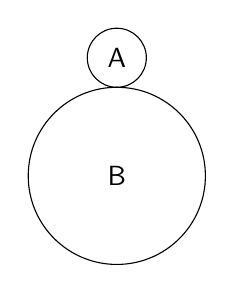
\begin{tikzpicture}[scale=.5]
    % Draw circle B (larger circle)
  \draw (0,0) circle (2.25cm);
    \node at (0,0) {B};
    
    % Draw circle A (smaller circle)
    \draw (0,3) circle (0.75cm);
    \node at (0,3) {A};
\end{tikzpicture}

\vspace{.5cm}

The radius of circle A is $\frac{1}{3}$ of the radius of circle B. Circle A rolls\\
around circle B one trip back to its starting point. How\\
many times will circle A revolve in total?

\vspace{.5cm}

\begin{tabular}{l@{\hspace{2em}}l@{\hspace{2em}}l@{\hspace{2em}}l@{\hspace{2em}}l}
  (a) $\frac{3}{2}$ & (b) 3 & (c) 6 & (d) $\frac{9}{2}$ & (e) 9
\end{tabular}
\end{center}

\vspace{.5cm}

\end{frame}

\section{Braess Paradox}

\begin{frame}

\end{frame}

\section{Voting Paradox}

\begin{frame}
  
  \begin{itemize}
    \item The Simplest Case
      \vspace{3mm}
      \begin{table}
        \center
        \begin{tabular}{cccc}
          \toprule
          \textbf{Voter} & \textbf{First preference} & \textbf{Second preference} & \textbf{Third preference} \\
          \midrule
          Voter 1 & A & B & C \\
          Voter 2 & B & C & A \\
          Voter 3 & C & A & B \\
          \bottomrule
        \end{tabular}
      \end{table}
      \vspace{3mm}
      \begin{center} A $>$ B $>$ C $>$ A \end{center}
      \vspace{1mm} 
    \item A More Complicated Situation
      \vspace{3mm}
      \begin{table}
        \center
        \begin{tabular}{llll}
          \toprule
          \textbf{Party} & \textbf{First preference} & \textbf{Second preference} & \textbf{Third preference} \\
          \midrule
          Left (3)   & education & health & security \\
          Center (4) & health & security & education \\
          Right (5)  & security & education & health \\
          \bottomrule
        \end{tabular}
      \end{table}
      \vspace{3mm}
        \begin{center} A $>$ B $>$ C $>$ A \end{center}
      \vspace{3mm} 
  \end{itemize}
\end{frame}

\section{Arrow's Impossibility Theorem}

\begin{frame}

\end{frame}

\section{St. Petersberg Paradox}

\begin{frame}{The Expected Utility Hypothesis}
\end{frame}

\begin{frame}{The Expected Utility Hypothesis}
  \begin{definition}
    The agent prefers the r.v. $X$ to r.v. $Y$ iff
    \begin{align*}
      \expc U(X) > \expc U(Y)
    \end{align*}
    where $\expc$ is the expectation operator, $U:\RR\mapsto\RR$ is the agent's utility function.
  \end{definition}
\end{frame}

\section{Allais Paradox}

\begin{frame}
  \begin{itemize}[<+->]\setlength\itemsep{0em}
    \item Game A
      \begin{align*}
        X = \begin{cases}101 & \text{prob. } 0.33\\100 & \text{prob. } 0.66\\ 0 & \text{prob. } 0.01 \end{cases} \qquad
        Y = 100 \;\text{ with prob. } 1
      \end{align*}
      \onslide<+->
      Mostly prefer $Y$ to $X$: from the Expected Utility Hypothesis 
      \onslide<+->
      \begin{multline}
        U(100) > 0.33\cdot U(101) + 0.66\cdot U(100) + 0.01\cdot U(0)\\ \ie 0.34\cdot U(100) > 0.33\cdot U(101) + 0.01\cdot U(0)
      \end{multline}
    \item Game B 
      \begin{align*}
        X = \begin{cases}100 & \text{prob. } 0.34\\ 0 & \text{prob. } 0.66 \end{cases} \qquad
        Y = \begin{cases}101 & \text{prob. } 0.33\\ 0 & \text{prob. } 0.67 \end{cases}
      \end{align*}
      \onslide<+->
      Mostly prefer $Y$ to $X$: from the Expected Utility Hypothesis 
      \onslide<+->
      \begin{multline}
        0.33\cdot U(101) + 0.67\cdot U(0) > 0.34\cdot U(100) + 0.66\cdot U(0)\\ \ie 0.33\cdot U(101) + 0.01\cdot U(0) > 0.34\cdot U(100)
      \end{multline}
  \end{itemize}
\end{frame}

\section{Ellsberg Paradox}

\begin{frame}
  \begin{itemize}[<+->]
    \item Given an urn with $30$ balls of colors red, yellow, and black
    \item There are $10$ red balls; total $20$ yellow / black balls, but the number of each type unknown
    \item The agent estimates the probability of drawing yellow as $p$ where $0 < p < \frac{2}{3}$
    \item A single ball is drawn from the urn
  \end{itemize}
\end{frame}

\begin{frame}
  \begin{itemize}[<+->]\setlength\itemsep{0em}
    \item Game A  
      \begin{align*}
        X = \begin{cases}100 & \text{if red}\\0 & \text{if yellow or black}\end{cases} \qquad
        Y = \begin{cases}100 & \text{if yellow}\\0 & \text{if red or black}\end{cases} \qquad
      \end{align*}
      \onslide<+->
      Mostly prefer $X$ to $Y$: from the Expected Utility Hypothesis 
      \onslide<+->
      \begin{multline}
        \frac{1}{3}\cdot U(100) + \frac{2}{3}\cdot U(0) > p\cdot U(100) + (1 - p)\cdot U(0) \\ \ie\big(\frac{1}{3} - p\big)\cdot U(100) > \big(\frac{1}{3} - p\big)\cdot U(0)
      \end{multline}
    \item Game B 
      \begin{align*}
        X = \begin{cases}100 & \text{if red or black}\\ 0 & \text{if yellow}\end{cases} \qquad
        Y = \begin{cases}100 & \text{if yellow or black}\\ 0 & \text{if red}\end{cases}
      \end{align*}
      \onslide<+->
      Mostly prefer $Y$ to $X$: from the Expected Utility Hypothesis 
      \onslide<+->
      \begin{multline}
        \frac{2}{3}\cdot U(100) + \frac{1}{3}\cdot U(0) > (1 - p)\cdot U(100) + p\cdot U(0) \\ \ie\big(\frac{1}{3} - p\big)\cdot U(0) > \big(\frac{1}{3} - p\big)\cdot U(100)
      \end{multline}
  \end{itemize}
\end{frame}

\end{document}
